\documentclass[11pt]{article}
\usepackage[margin=1.1in]{geometry}
\usepackage{amsmath,amssymb,amsthm,booktabs,graphicx,hyperref,longtable}
\newtheorem{theorem}{Theorem}[section]
\newtheorem{lemma}[theorem]{Lemma}
\newtheorem{corollary}[theorem]{Corollary}
\newtheorem{proposition}[theorem]{Proposition}
\newtheorem{conjecture}[theorem]{Conjecture}
\theoremstyle{remark}
\newtheorem{remark}[theorem]{Remark}
\newcommand{\E}{\mathbb{E}}
\newcommand{\R}{\mathbb{R}}
\newcommand{\Z}{\mathbb{Z}}
\newcommand{\vol}{\operatorname{vol}}
\newcommand{\Cat}{\operatorname{Cat}}
\newcommand{\PP}{\mathcal{P}_2}
\newcommand{\gT}{\gamma_T}
\newcommand{\gH}{\gamma_H}

\title{Exact higher moments of the limiting spectral distributions\\
of random Toeplitz and Hankel matrices}
\author{Yitzchak Shmalo$^{\,a}$\thanks{Email address:
\texttt{yitzchak.shmalo@gmail.com} (Yitzchak Shmalo). Code and complete data
accompany this paper; see Section~\ref{sec:repro}.}\\[2pt]
{\small $^{a}$Einstein Institute of Mathematics, The Hebrew University of
Jerusalem, Givat Ram,}\\[-2pt]
{\small Jerusalem, Israel}}
\date{June 10, 2026}

\begin{document}
\maketitle

\begin{abstract}
The limiting spectral distributions $\gT$ and $\gH$ of random symmetric Toeplitz and
Hankel matrices (Bryc--Dembo--Jiang, \emph{Ann.\ Probab.}\ 34 (2006); Hammond--Miller,
\emph{J.\ Theoret.\ Probab.}\ 18 (2005)) have been known to exist for two decades, yet
remain unidentified; their explicitly published moments stop at order eight. We compute
the moments exactly through order $14$ for both ensembles, in exact rational
arithmetic:
$m_{10}(\gT)=415$, $m_{12}(\gT)=23840/7$, $m_{14}(\gT)=325719/10$,
$m_{10}(\gH)=2717/36$, $m_{12}(\gH)=1052/3$, $m_{14}(\gH)=1331087/720$. The
computation also yields $m_8(\gT)=908/15$, correcting the value $964/15$ reported by
Hammond--Miller. Each moment is a sum of
volumes of explicit rational polytopes indexed by pair partitions; we evaluate every
volume exactly by a double-description/triangulation engine and check the results
against an independent vertex enumeration, Monte Carlo integration, direct eigenvalue
simulation, an exact counting route, and all previously published values.
We further prove a sharp structural theorem: a pairing has volume $1$ if and only if
it is non-crossing, and every crossing pairing has volume at most $2/3$ --- attained
in the Toeplitz case --- in both ensembles; consequently
$m_{2k}(\gT)\le \Cat_k+\tfrac23\big((2k-1)!!-\Cat_k\big)$ and
$m_{2k}(\gH)\le \Cat_k+\tfrac23\big(k!-\Cat_k\big)$. The complete volume spectra are
tabulated, in the paper and in the accompanying repository; they are supported on a
small set of rational values, shared across the two ensembles. We close with two numerical observations: the Gaussian-deficit ratios of
$\gT$ trend toward the square of the Sen--Vir\'ag spectral-norm constant, and the
analogous Hankel ratios suggest a value for the (open) Hankel norm constant.
\end{abstract}

\section{Introduction}

Let $\{a_j\}_{j\ge 0}$ be i.i.d.\ real random variables with $\E a_0=0$, $\E a_0^2=1$
and all moments finite. The random symmetric Toeplitz and Hankel matrices are
\[
T_n=\big(a_{|i-j|}\big)_{i,j=0}^{n-1},\qquad
H_n=\big(a_{i+j}\big)_{i,j=0}^{n-1}.
\]
Bryc, Dembo and Jiang \cite{BDJ} and Hammond and Miller \cite{HM} proved that the
empirical spectral distributions of $T_n/\sqrt n$ and $H_n/\sqrt n$ converge weakly,
almost surely, to nonrandom symmetric probability measures $\gT$, $\gH$ that do not
depend on the entry law. Both measures have unbounded support; $\gH$ is not unimodal
\cite{BDJ}; $\gT$ is absolutely continuous with bounded density \cite{SV1}; the spectral
norm of $T_n$ obeys $\|T_n\|/\sqrt{2n\log n}\to 0.8288\ldots$ \cite{Meckes,SV2}.
Identifying $\gT$ or $\gH$ in closed form is a recognized open problem: already the
2003 review \cite{BoseReview} noted of the then-new existence result that ``its
closed form is not yet known'', and two decades later the laws remain unidentified.
Recent work provides alternative \emph{representations} of the limits --- moment
formulas for dependent-entry generalizations that include the i.i.d.\ case
\cite{Maurya}, and a description via $*$-convergence of circulant-type matrices
\cite{BoseVish} --- without producing closed forms or explicit higher moments. The
only explicitly published moment values are
\[
m_4(\gT)=\tfrac83,\quad m_6(\gT)=11,\quad m_8(\gT)\ \text{(see below)},\qquad
m_4(\gH)=2,\quad m_6(\gH)=\tfrac{11}2,\quad m_8(\gH)=\tfrac{281}{15}.
\]

Since both limit laws are symmetric and determined by their moments \cite{BDJ}, exact
higher moments are the natural invariants through which these unidentified laws can be
studied, compared against candidate closed forms, and reconstructed numerically. This
paper contributes:

\begin{enumerate}
\item \textbf{New exact moments} (Theorem~\ref{thm:values}): $m_{10}(\gT)=415$,
$m_{12}(\gT)=\tfrac{23840}{7}$, $m_{14}(\gT)=\tfrac{325719}{10}$,
$m_{10}(\gH)=\tfrac{2717}{36}$, $m_{12}(\gH)=\tfrac{1052}{3}$,
$m_{14}(\gH)=\tfrac{1331087}{720}$, all in exact rational arithmetic, with the
complete volume spectrum of every order tabulated (Section~\ref{sec:results} and the
data repository).
\item \textbf{A correction}: the eighth Toeplitz moment is
$m_8(\gT)=\tfrac{908}{15}=60.5\overline{3}$, while \cite{HM} reports
$64\tfrac4{15}=\tfrac{964}{15}$; Section~\ref{sec:correction} gives the configuration
count behind the corrected value, in the format of \cite{HM}, together with the
verifications.
\item \textbf{A sharp structural theorem}
(Theorem~\ref{thm:gap}): in both ensembles the polytope volume attached to a pair
partition equals $1$ exactly when the pairing is non-crossing, and is at most $2/3$
otherwise --- with $2/3$ attained (Toeplitz). This yields explicit upper bounds for
\emph{all} moments (Corollary~\ref{cor:bound}) and explains the leading structure of
the moment sequences.
\item \textbf{Quantitative consequences} (Section~\ref{sec:consequences}): explicit
tail bounds; Gaussian-deficit sequences; and two numerical observations, connecting
the deficit ratios of $\gT$ to the Sen--Vir\'ag constant $0.8289$ and suggesting an
estimate for the unknown Hankel norm constant.
\end{enumerate}

\section{The moment--volume formulas}\label{sec:formulas}

We recall and re-derive the volume representation of the limit moments, in the precise
normalization used by our computations. Let $\PP(2k)$ denote the perfect matchings
(\emph{pairings}) of $\{0,1,\dots,2k-1\}$; $|\PP(2k)|=(2k-1)!!$. For
$\pi\in\PP(2k)$ write $\pi=\{\{l_1,m_1\},\dots,\{l_k,m_k\}\}$ with $l_c<m_c$, let
$v(r)$ be the index of the pair containing slot $r$, and say $\pi$ is
\emph{parity-mixing} if every pair joins an even and an odd slot.

\begin{theorem}[essentially \cite{BDJ,HM}]\label{thm:volumes}
For $t=(t_1,\dots,t_k)\in\R^k$ define
$S_l(t)=\sum_{r<l}\sigma(r)\,t_{v(r)}$, where $\sigma(r)=+1$ if $r$ is the smaller
element of its pair and $-1$ otherwise. Let
\[
P_\pi=\Big\{(x_0,t)\in\R^{k+1}:\ 0\le x_0+S_l(t)\le 1,\ l=0,1,\dots,2k-1\Big\},
\qquad p_T(\pi)=\vol_{k+1}(P_\pi).
\]
Then $m_{2k}(\gT)=\sum_{\pi\in\PP(2k)}p_T(\pi)$.

For parity-mixing $\pi$ define
$A_l(x_0,y)=(-1)^l x_0+\sum_{r<l}(-1)^{l-1-r}y_{v(r)}$ and
\[
P^H_\pi=\Big\{(x_0,y)\in\R^{k+1}:\ 0\le A_l(x_0,y)\le 1,\ l=0,\dots,2k-1\Big\},
\qquad p_H(\pi)=\vol_{k+1}(P^H_\pi).
\]
Then $m_{2k}(\gH)=\sum_{\pi\ \mathrm{parity\hbox{-}mixing}}p_H(\pi)$, the sum having
$k!$ terms.
\end{theorem}

\begin{proof}
Expanding $\E\operatorname{tr} T_n^{2k}$ over closed index circuits
$(i_0,\dots,i_{2k-1})$, the slot values are $d_l=i_{l+1}-i_l$ (indices mod $2k$),
$\sum_l d_l=0$. Independence and centering force every value of $|d_l|$ to occur at
least twice; configurations with fewer than $k$ distinct values are $O(n^{k})$ in
number against the normalization $n^{-(k+1)}$, hence vanish in the limit, leaving pair
partitions with $\E a^2=1$ per pair. For a matched pair $\{l,m\}$, $d_m=\pm d_l$; if
$d_m=+d_l$ for some pair, the closure $\sum_l d_l=0$ becomes a nontrivial linear
constraint on the $k$ free differences, again $O(n^{k})$. So at leading order
$d_{m_c}=-d_{l_c}$ for all pairs, and the circuit is determined by $i_0$ and the $k$
values $x_c:=d_{l_c}$, subject to $i_l=i_0+\sum_{r<l}\sigma(r)x_{v(r)}\in[0,n)$ for all
$l$. Scaling $x_0=i_0/n$, $t_c=x_c/n$ and letting $n\to\infty$, the normalized count is
a Riemann sum converging to $\vol(P_\pi)$ (the constraints $t_c\in[-1,1]$ being implied
by consecutive slot constraints). Boundary strata ($x_c=0$, ties $|x_c|=|x_{c'}|$,
diagonal entries) have codimension $\ge1$ and do not contribute. Convergence of
$\E$-moments plus the concentration proved in \cite{BDJ} upgrades this to the moments
of $\gT$.

For Hankel the slot values are $s_l=i_l+i_{l+1}$, whence
$i_l=(-1)^l i_0+\sum_{r<l}(-1)^{l-1-r}s_r$ and the closure constraint
$\sum_r(-1)^r s_r=0$. Matching $s$-values in pairs, the closure is automatic precisely
for parity-mixing pairings and a nontrivial constraint otherwise (one degree of freedom
lost, hence negligible). Scaling $y_c=s_{l_c}/n\in[0,2]$ gives the stated polytope; the
bounds $y_c\in[0,2]$ are implied by consecutive constraints.
\end{proof}

\begin{remark}
$P_\pi$ is cut out by at most $4k$ halfspaces with coefficients in $\{-1,0,1\}$ and
right-hand sides in $\{0,1\}$, so $p_T(\pi),p_H(\pi)\in\mathbb{Q}$. The first values:
$m_2=1$ for both ensembles; $m_4(\gT)=1+1+\tfrac23=\tfrac83$; $m_4(\gH)=1+1=2$.
\end{remark}

\subsection{Symmetries and reductions}

\begin{lemma}[dihedral invariance]\label{lem:dihedral}
$p_T$ and $p_H$ are constant on orbits of the dihedral group $D_{2k}$ acting on slots
(rotations $r\mapsto r+1$ and reflections $r\mapsto c-r$ mod $2k$; for Hankel both
operations preserve the parity-mixing class).
\end{lemma}
\begin{proof}
The set of admissible circuits $\{(i_0,\dots,i_{2k-1})\}$ counted in the proof of
Theorem~\ref{thm:volumes} is intrinsic to the cyclic word
$a_{w(i_0,i_1)}a_{w(i_1,i_2)}\cdots a_{w(i_{2k-1},i_0)}$ ($w(i,j)=|i-j|$ resp.\ $i+j$):
relabeling the circuit cyclically or reversing its orientation maps admissible circuits
for $\pi$ bijectively onto those for the transformed pairing. The volume is the
$n\to\infty$ normalized count, hence equal.
\end{proof}

\begin{lemma}[adjacent-pair deletion]\label{lem:deletion}
If $\pi$ pairs two adjacent slots $\{l,l+1\}$, deleting them (and relabeling) yields
$\pi'\in\PP(2k-2)$ with $p(\pi)=p(\pi')$, in both ensembles.
\end{lemma}
\begin{proof}
The pair's variable appears in exactly one constraint, $0\le x_0+S_l\pm t\le1$ (resp.\
$0\le y-A_l\le 1$), and in no other; given the remaining variables the constraint
confines it to an interval of length exactly $1$ contained in its implied range.
Fubini integrates it out with factor $1$.
\end{proof}

Since every non-crossing pairing contains an adjacent pair, induction gives:

\begin{corollary}\label{cor:nc1}
$p_T(\pi)=p_H(\pi)=1$ for every non-crossing $\pi$. (Every non-crossing pairing is
parity-mixing, so all $\Cat_k=\binom{2k}{k}/(k+1)$ of them appear in both ensembles.)
\end{corollary}

\section{Volume $1$ characterizes non-crossing pairings, with a $2/3$ gap}

Throughout this section fix $\pi\in\PP(2k)$ with pairs $\{l_c,m_c\}$, $l_c<m_c$,
labelled so that $l_1<l_2<\dots<l_k$. Write
\[
O(l):=\{c:\ l_c<l\le m_c\}\qquad\text{(the pairs \emph{open} at slot $l$)},
\qquad l=0,1,\dots,2k .
\]

\begin{lemma}[opening-slot coordinates, Toeplitz]\label{lem:coords}
Let $W_l=x_0+S_l(t)$ for $l=0,\dots,2k-1$, so that
$P_\pi=\{(x_0,t):W_l\in[0,1]\ \forall l\}$. Then:
(i) $W_l=x_0+\sum_{c\in O(l)}t_c$ for every $l$;
(ii) the linear map $\Phi:(x_0,t_1,\dots,t_k)\mapsto(W_0,W_{l_1+1},\dots,W_{l_k+1})$
is unimodular, i.e.\ $\det\Phi=\pm1$;
(iii) every $W_l$ expands uniquely as an integer combination of the \emph{basis}
coordinates $\Phi_0:=W_0$, $\Phi_c:=W_{l_c+1}$ ($1\le c\le k$), with no constant
term, and the coefficients $(\alpha_i)$ of any such expansion satisfy
$\sum_i\alpha_i=1$.
\end{lemma}

\begin{proof}
(i) In $S_l=\sum_{r<l}\sigma(r)t_{v(r)}$, a pair $c$ with $m_c<l$ contributes
$t_c-t_c=0$, a pair with $l_c<l\le m_c$ contributes $+t_c$, and later pairs
contribute nothing. (ii) $W_0=x_0$ and
$W_{l_c+1}=x_0+t_c+\sum_{c'\in O(l_c+1),\,c'\neq c}t_{c'}$, where every
$c'\in O(l_c+1)\setminus\{c\}$ has $l_{c'}<l_c$; in the variable order
$(x_0,t_1,\dots,t_k)$ the matrix of $\Phi$ is lower triangular with unit diagonal.
(iii) Unimodularity gives unique integral expansions; all the forms involved are
homogeneous linear in $(x_0,t)$, so no constant appears, and comparing the
coefficient of $x_0$ on both sides of $W_l=\sum_i\alpha_i\Phi_i$ (each $\Phi_i$ has
$x_0$-coefficient $1$, as does $W_l$) gives $\sum_i\alpha_i=1$.
\end{proof}

\begin{lemma}[crossings force a thick slot]\label{lem:thick}
If $\pi$ has a crossing, some slot $l^*\in\{1,\dots,2k-1\}$ has an expansion
$W_{l^*}=\sum_i\alpha_i\Phi_i$ with at least two nonzero coefficients.
\end{lemma}

\begin{proof}
By Lemma~\ref{lem:coords}(i), the expansion of $W_l$ has exactly one nonzero
coefficient iff $W_l$ equals some basis form: $W_l=\Phi_0$ iff $O(l)=\emptyset$, and
$W_l=\Phi_c$ iff $O(l)=O(l_c+1)$ (two homogeneous forms $x_0+\sum_{O}t$,
$x_0+\sum_{O'}t$ agree iff $O=O'$; a relation $W_l=-\Phi_i$ or
$W_l=\alpha\Phi_i$ with $\alpha\neq1$ is impossible by the $x_0$-coefficient).
Suppose, for contradiction, that for every $l$ the open set $O(l)$ is $\emptyset$ or
equals $O(l_c+1)$ for some $c$.

Let $m^*$ be the first slot that closes a pair $\alpha$ while some pair $\beta$
opened after $\alpha$ is still open; $m^*$ exists because $\pi$ has a crossing
(take the first slot at which a crossing pair closes). Set $O:=O(m^*+1)$. Then
$\beta\in O$, $\alpha\notin O$, so $O\neq\emptyset$, and $m^*+1\le 2k-1$ (were
$m^*=2k-1$, nothing would remain open after it). We show $O\neq O(l_c+1)$ for every
$c$, the desired contradiction:
\begin{itemize}
\item If $l_c+1\le m^*$: at every slot $\le m^*$ at which $\beta$ is open, $\alpha$
is open as well ($\alpha$ opened before $\beta$ and does not close until $m^*$). So
if $\beta\in O(l_c+1)$ then $\alpha\in O(l_c+1)$, while $\alpha\notin O$; and if
$\beta\notin O(l_c+1)$ then $O(l_c+1)\ne O$ directly. Either way $O(l_c+1)\neq O$.
\item If $l_c+1>m^*+1$: the pair $c$ belongs to $O(l_c+1)$ and opened at
$l_c>m^*$; but every pair of $O$ is open at $m^*+1$, hence opened before $m^*+1$.
So $c\in O(l_c+1)\setminus O$ and $O(l_c+1)\neq O$. (The case $l_c+1=m^*+1$ cannot
occur: $m^*$ is a closing slot.)
\end{itemize}
\end{proof}

\begin{lemma}[window bound]\label{lem:window}
Let $r\ge2$, let $\alpha_1,\dots,\alpha_r$ be nonzero integers with
$\sum_i\alpha_i=1$, let $U_1,\dots,U_r$ be i.i.d.\ $\mathrm{Unif}[0,1]$, and let
$I$ be any interval of length $1$. Then
\[
\mathbb{P}\Big(\sum_{i=1}^r\alpha_iU_i\in I\Big)\ \le\ \tfrac23 ,
\]
with equality when $r=3$, $(\alpha_i)=(1,1,-1)$ and $I=[0,1]$.
\end{lemma}

\begin{proof}
If some $|\alpha_j|\ge2$: conditionally on the other variables, $\alpha_jU_j$ is
uniform on an interval of length $\ge2$, so it lands in any unit window with
probability $\le\tfrac12$; integrating, the mass is $\le\tfrac12$.

If all $|\alpha_i|=1$: $r$ must be odd (a sum of $r$ odd numbers has the parity of
$r$, and it equals $1$), so $r\ge3$. Each $-U_i$ equals $U_i'-1$ with
$U_i'=1-U_i\sim\mathrm{Unif}[0,1]$, so $\sum\alpha_iU_i$ is a shift of an
Irwin--Hall sum $\Sigma_r$ of $r$ uniforms, whose density $f_r$ is symmetric and
unimodal. For $r=3$: the best unit window is the central one, and
$\mathbb{P}(\Sigma_3\in[1,2])=1-2\,\mathbb{P}(\Sigma_3<1)=1-\tfrac26=\tfrac23$
(each tail is a corner simplex of volume $1/6$); for the sign pattern $(1,1,-1)$
and $I=[0,1]$ this is attained exactly. For odd $r\ge5$:
$\sup f_r=f_r(r/2)\le f_5(5/2)=\tfrac{115}{192}<\tfrac23$, so any unit window has
mass $<\tfrac23$. (The central values decrease in $r$: since
$f_{r+1}=f_r\ast\mathbf{1}_{[0,1]}$ we have
$f_{r+1}\big(\tfrac{r+1}{2}\big)=\int_{r/2-1/2}^{r/2+1/2}f_r(x)\,dx\le\sup f_r
=f_r\big(\tfrac{r}{2}\big)$, the last equality by symmetry and unimodality;
$f_5(5/2)=\tfrac{115}{192}$ is the standard Irwin--Hall evaluation.)
\end{proof}

\begin{lemma}[opening-slot coordinates, Hankel]\label{lem:coordsH}
Let $\pi$ be parity-mixing and $B_l:=(-1)^lA_l$. Then
$B_l=x_0+\sum_{c\in O(l)}\varepsilon_c\,y_c$ with fixed signs
$\varepsilon_c=-(-1)^{l_c}$; the map
$(x_0,y)\mapsto(B_0,B_{l_1+1},\dots,B_{l_k+1})$ is unimodular; the constraint on
$B_l$ is the unit window $[0,1]$ ($l$ even) or $[-1,0]$ ($l$ odd); and the
conclusions (iii) of Lemma~\ref{lem:coords} and Lemma~\ref{lem:thick} hold verbatim
with $\Phi_c=B_{l_c+1}$ and the signed variables $\varepsilon_cy_c$ in place of
$t_c$.
\end{lemma}

\begin{proof}
$A_{l+1}=s_l-A_l$ gives $B_{l+1}=(-1)^{l+1}(s_l-A_l)=B_l+(-1)^{l+1}s_l$, so
$B_l=x_0-\sum_{r<l}(-1)^r s_r$; for a closed pair ($m_c<l$) the two appearances of
$y_c$ carry opposite signs $(-1)^{l_c},(-1)^{m_c}$ and cancel \emph{because} $\pi$
is parity-mixing, leaving exactly the open pairs with the stated signs.
Unimodularity is the same triangular structure as in Lemma~\ref{lem:coords}(ii)
(the diagonal entries are $\varepsilon_c=\pm1$). The open-set argument of
Lemma~\ref{lem:thick} uses only the combinatorics of $O(\cdot)$ and the
$x_0$-coefficients, not the signs, so it transfers verbatim: signed open sums
$x_0+\sum_O\varepsilon y$ and $x_0+\sum_{O'}\varepsilon y$ agree as forms iff
$O=O'$ (each pair's sign is fixed once and for all).
\end{proof}

\begin{theorem}\label{thm:gap}
Let $\pi\in\PP(2k)$ (parity-mixing in the Hankel case). If $\pi$ has a crossing, then
\[
p_T(\pi)\le\tfrac23,\qquad p_H(\pi)\le\tfrac23 ,
\]
and $2/3$ is attained in the Toeplitz case (by the one-crossing pairing, arbitrarily
padded with non-crossing material). Hence $p(\pi)=1$ if and only if $\pi$ is
non-crossing, in both ensembles, and $\sup_{\pi\ \mathrm{crossing}}p_T(\pi)=\tfrac23$.
\end{theorem}

\begin{proof}
\emph{Toeplitz.} By Lemma~\ref{lem:coords}(ii), $p_T(\pi)$ equals the volume of
$\Phi(P_\pi)$. Among its defining constraints are the $k+1$ basis-cube constraints
$\Phi_i\in[0,1]$ and, by Lemma~\ref{lem:thick}, a constraint
$\sum_i\alpha_i\Phi_i\in[0,1]$ whose integer coefficients are $\ge2$ in number,
nonzero, and sum to $1$ (Lemma~\ref{lem:coords}(iii)). Discarding all other
constraints and applying Fubini on the cube,
\[
p_T(\pi)\ \le\ \mathbb{P}\Big(\sum_i\alpha_iU_i\in[0,1]\Big)\ \le\ \tfrac23
\]
by Lemma~\ref{lem:window}. \emph{Sharpness:} for $\pi^\times=\{0,2\},\{1,3\}$ the
image polytope is exactly
$\{(\Phi_0,\Phi_1,\Phi_2)\in[0,1]^3:\Phi_0-\Phi_1+\Phi_2\in[0,1]\}$ (four
constraints in total), whose volume is the equality case of
Lemma~\ref{lem:window}: $p_T(\pi^\times)=\tfrac23$. By
Lemmas~\ref{lem:dihedral}--\ref{lem:deletion}, inserting non-crossing material
preserves this value, so volume-$\tfrac23$ crossing pairings exist for every
$k\ge2$.

\emph{Hankel.} By Lemma~\ref{lem:coordsH}, $p_H(\pi)$ is the volume of a polytope
whose constraints include $k+1$ unit-window constraints on the basis coordinates
and one constraint $\sum_i\alpha_i B_i\in J$ ($J$ a unit window) with $r\ge2$
nonzero integer coefficients. Recentring each basis coordinate to
$\mathrm{Unif}[0,1]$ translates $J$ by an integer; Lemma~\ref{lem:window} covers
\emph{arbitrary} unit windows, so $p_H(\pi)\le\tfrac23$.

In both ensembles, Corollary~\ref{cor:nc1} gives $p=1$ on non-crossing pairings,
completing the equivalence.
\end{proof}

\begin{corollary}\label{cor:bound}
For all $k\ge1$,
\[
m_{2k}(\gT)\ \le\ \Cat_k+\tfrac23\big((2k-1)!!-\Cat_k\big),\qquad
m_{2k}(\gH)\ \le\ \Cat_k+\tfrac23\big(k!-\Cat_k\big),
\]
and (by Corollary \ref{cor:nc1}) $m_{2k}\ge\Cat_k$ in both ensembles.
\end{corollary}

\begin{remark}\label{rem:hankel-half}
The Toeplitz bound is sharp pairing-by-pairing (Theorem~\ref{thm:gap}). For Hankel the
largest crossing volume in all computed data (through order $14$, i.e.\ all
$7!=5040$ parity-mixing pairings and everything below) is $\tfrac12$; we conjecture
$\sup_{\pi\ \mathrm{crossing}}p_H(\pi)=\tfrac12$ --- the parity-mixing constraint
excludes the $r=3$ centred-window configuration that achieves $2/3$ in the Toeplitz
case (the one-crossing pairing $\{0,2\},\{1,3\}$ is not parity-mixing).
\end{remark}

\section{Exact computation and verification}\label{sec:computation}

\subsection{Algorithm}
For each dihedral orbit representative (Lemma~\ref{lem:dihedral}; e.g.\ $10395$
pairings reduce to $554$ orbits at $2k=12$) we evaluate $\vol(P_\pi)$ exactly:
(i) the $\le4k$ halfspaces (integer data) are deduplicated;
(ii) vertices are enumerated by incremental \emph{double description} over
$\mathbb{Q}$, starting from the bounding box, with the standard combinatorial
adjacency criterion;
(iii) the polytope is triangulated combinatorially: faces are identified with their
sets of incident vertices via exact tight-set masks, facets of a face are detected by
exact affine-rank tests, and each face is coned from its minimal vertex;
(iv) the volume is $\sum|\det|/d!$ over the resulting simplices, in exact rational
arithmetic. The implementation is $\sim$300 lines of dependency-free Python
(\texttt{exact\_volume.py}); $2k=12$ (Toeplitz) takes under two minutes on 14 cores,
and the largest run --- $2k=14$, Toeplitz: $135135$ pairings in $5283$ dihedral
orbits --- about $90$ minutes.

\subsection{Verification}\label{sec:verification}
Because our value differs from a published one, we checked the pipeline in several
independent ways:
\begin{enumerate}
\item \emph{Published values.} The engine reproduces exactly $m_4(\gT)=8/3$,
$m_6(\gT)=11$ (including Hammond--Miller's configuration data
$2,6,3,3,1\times$ volumes $1,\tfrac23,1,\tfrac12,\tfrac12$), $m_4(\gH)=2$,
$m_6(\gH)=\tfrac{11}{2}$, and $m_8(\gH)=\tfrac{281}{15}$ \cite{BDJ,HM}.
\item \emph{Independent vertex enumeration.} For every orbit at order $8$ (both
ensembles), brute-force enumeration over all $\binom{m}{d}$ constraint subsets
reproduces the DD vertex sets exactly, and the float convex-hull volume
(\texttt{scipy}/Qhull, an independent triangulation) matches each exact volume to
$10^{-10}$.
\item \emph{Per-orbit Monte Carlo.} Every orbit volume at every computed order was
checked by vectorized rejection sampling ($10^6$; at order $8$, $10^8$ samples per
orbit): all $z$-scores lie in $[-2,2]$. For the disputed total this gives
$m_8(\gT)=60.544\pm0.0086$, i.e.\ the published $964/15=64.267$ is rejected at
$432\sigma$ while $908/15=60.533$ agrees at $1.2\sigma$.
\item \emph{Eigenvalue simulation.} Empirical spectral moments of simulated matrices
($n=1000,2000,4000$; $320/96/28$ repetitions) extrapolated linearly in $1/n$ agree with
every exact value; e.g.\ $m_8(\gT)$: $60.87\pm2.51$; $m_{10}(\gT)$: $416\pm34$ (exact
$415$); $m_{12}(\gT)$: $3384\pm535$ (exact $3405.7$); $m_{12}(\gH)$: $332\pm18$ (exact
$350.7$, $1\sigma$); $m_{10}(\gH)$: $74.4\pm2.3$ (exact $75.47$).
\item \emph{Independent exact counting.} For Rademacher entries,
$\E\operatorname{tr}(A_n/\sqrt n)^{2k}/n$ is an exactly computable integer count
(circuits whose slot-value multiset has all even multiplicities), evaluated by a
meet-in-the-middle dynamic program with multiset parity tracked through $127$-bit
hashing, and is an Ehrhart-type quasi-polynomial in $n$. For Hankel, interpolation
through $n\in\{4,\dots,14\}$ with held-out exact prediction at $n=16,18$ recovers
$m_6(\gH)=\tfrac{11}2$ and $m_8(\gH)=\tfrac{281}{15}$ \emph{exactly} --- validating the
counting route --- while the Toeplitz counts converge too slowly at these $n$ for naive
interpolation; a three-term fit of the Toeplitz counts at $n=14,16,18$ extrapolates
to $\approx61.5$, consistent with $908/15$ and not with $964/15$.
\item \emph{Internal consistency.} Orbit-constancy of volumes (Lemma~\ref{lem:dihedral})
was verified on random orbit members at every order; the volume-$1$ pairings in every
dataset are exactly the non-crossing ones, $\Cat_k$ in number
(Theorem~\ref{thm:gap}); brute-force summation over all $105$ pairings at $2k=8$
(no symmetry reduction) reproduces $908/15$.
\end{enumerate}
These checks differ in logical strength. Items 1--4 and 6 bear directly
on the disputed value: two exact independent computations of the same polytope data
(double description vs.\ brute-force basis enumeration), an independent float
triangulation, a $432\sigma$ Monte Carlo discrimination, and direct eigenvalue
simulation. Item 5 is an \emph{exact} independent route where it terminates (the
Hankel controls at orders $6$ and $8$) and a consistency check --- not an exact
verification --- for the Toeplitz value, whose finite-$n$ counts converge too slowly
for interpolation at accessible sizes.

\section{Results}\label{sec:results}

\begin{theorem}\label{thm:values}
The even moments of the Toeplitz and Hankel limiting spectral distributions are
\begin{center}
\begin{tabular}{c|cc|cc}
\toprule
$2k$ & $m_{2k}(\gT)$ & numeric & $m_{2k}(\gH)$ & numeric\\
\midrule
2  & $1$ & $1$ & $1$ & $1$\\
4  & $8/3$ & $2.6667$ & $2$ & $2$\\
6  & $11$ & $11$ & $11/2$ & $5.5$\\
8  & $\mathbf{908/15}$ & $60.5333$ & $281/15$ & $18.7333$\\
10 & $\mathbf{415}$ & $415$ & $\mathbf{2717/36}$ & $75.4722$\\
12 & $\mathbf{23840/7}$ & $3405.7143$ & $\mathbf{1052/3}$ & $350.6667$\\
14 & $\mathbf{325719/10}$ & $32571.9$ & $\mathbf{1331087/720}$ & $1848.7319$\\
\bottomrule
\end{tabular}
\end{center}
Bold values are new (the bold $m_8$ corrects \cite{HM}); odd moments vanish.
\end{theorem}

\subsection{Volume spectra}
The volumes take few distinct rational values, shared across ensembles
(consequences of Lemmas~\ref{lem:dihedral}--\ref{lem:deletion}: padding a ``core''
crossing diagram with non-crossing material preserves its volume).

\medskip
\noindent\textbf{Toeplitz.}
\begin{center}
\small
\begin{tabular}{c|l}
\toprule
$2k$ & volume $\times$ number of pairings\\
\midrule
4 & $1\times2$;\ $\tfrac23\times1$\\
6 & $1\times5$;\ $\tfrac23\times6$;\ $\tfrac12\times4$\\
8 & $1\times14$;\ $\tfrac23\times28$;\ $\tfrac12\times32$;\ $\tfrac9{20}\times4$;\
$\tfrac25\times5$;\ $\tfrac{11}{30}\times22$\\
10 & $1\times42$;\ $\tfrac23\times120$;\ $\tfrac12\times180$;\ $\tfrac9{20}\times40$;\
$\tfrac49\times5$;\ $\tfrac25\times50$;\ $\tfrac{11}{30}\times220$;\
$\tfrac{61}{180}\times40$;\ $\tfrac13\times6$;\ $\tfrac{13}{45}\times70$;\
$\tfrac{49}{180}\times150$;\ $\tfrac14\times22$\\
\bottomrule
\end{tabular}
\end{center}
(the $2k=12$ spectrum, with $554$ orbits and $28$ distinct volumes, is in
Appendix~\ref{app:spectra}).

\medskip
\noindent\textbf{Hankel.}
\begin{center}
\small
\begin{tabular}{c|l}
\toprule
$2k$ & volume $\times$ number of pairings\\
\midrule
4 & $1\times2$\\
6 & $1\times5$;\ $\tfrac12\times1$\\
8 & $1\times14$;\ $\tfrac12\times8$;\ $\tfrac{11}{30}\times2$\\
10 & $1\times42$;\ $\tfrac12\times45$;\ $\tfrac{11}{30}\times20$;\ $\tfrac13\times1$;\
$\tfrac{13}{45}\times5$;\ $\tfrac{49}{180}\times5$;\ $\tfrac14\times2$\\
12 & $1\times132$;\ $\tfrac12\times220$;\ $\tfrac{11}{30}\times132$;\ $\tfrac13\times12$;\
$\tfrac{13}{45}\times60$;\ $\tfrac{49}{180}\times60$;\ $\tfrac{23}{90}\times6$;\
$\tfrac14\times24$;\ $\tfrac5{21}\times6$;\ $\tfrac{68}{315}\times12$;\
$\tfrac{29}{140}\times2$;\ $\tfrac{509}{2520}\times36$;\ $\tfrac{239}{1260}\times12$;\
$\tfrac{19}{105}\times6$\\
\bottomrule
\end{tabular}
\end{center}

Note the volume-$1$ counts $2,5,14,42,132$: the Catalan numbers, as proved in
Theorem~\ref{thm:gap}.

\subsection{The eighth Toeplitz moment: correction of Hammond--Miller}
\label{sec:correction}
At $2k=8$ the $105$ pairings split into $17$ dihedral orbits carrying six distinct
volumes; grouping by volume:
\[
m_8(\gT)=14\cdot1+28\cdot\tfrac23+32\cdot\tfrac12+4\cdot\tfrac9{20}
+5\cdot\tfrac25+22\cdot\tfrac{11}{30}
=14+\tfrac{56}3+16+\tfrac95+2+\tfrac{121}{15}=\tfrac{908}{15},
\]
i.e.\ $60\tfrac8{15}$, in place of the $64\tfrac4{15}$ of \cite{HM}. The
multiplicities above sum to $105$, and every individual volume is verified by the
methods of Section~\ref{sec:verification}. All other values of \cite{HM}, including
$m_6=11$ with its configuration table, are confirmed by our computation.

\section{Consequences and observations}\label{sec:consequences}

\subsection{Gaussian and factorial deficits}
Write $\delta^T_k=m_{2k}(\gT)/(2k-1)!!$ (Gaussian deficit) and
$\delta^H_k=m_{2k}(\gH)/k!$ (deficit against the symmetrized-Rayleigh/reverse-circulant
moments $k!$):
\[
\delta^T:\ 1,\ \tfrac89,\ \tfrac{11}{15},\ \tfrac{908}{1575},\ \tfrac{83}{189},\
\tfrac{4768}{14553},\ \tfrac{36191}{150150}
\qquad
\delta^H:\ 1,\ 1,\ \tfrac{11}{12},\ \tfrac{281}{360},\ \tfrac{2717}{4320},\
\tfrac{263}{540},\ \tfrac{1331087}{3628800}.
\]
Both decrease strictly from $k=2$ resp.\ $3$ on (consistent with
Theorem~\ref{thm:gap}); the successive ratios $\delta_k/\delta_{k-1}$ are
\[
\text{Toeplitz ($k=2..7$): } .8889,\ .8250,\ .7861,\ .7617,\ .7461,\ .7357,
\qquad
\text{Hankel ($k=3..7$): } .9167,\ .8515,\ .8058,\ .7744,\ .7532 .
\]

\subsection{Numerical observations: deficit ratios and norm constants}
\emph{Everything in this subsection is heuristic extrapolation from the exact data;
nothing here is proved, and none of the results elsewhere in the paper depend on it.}
If $m_{2k}\approx C\,(2k-1)!!\,\sigma_*^{2k}$ for large $k$ --- the moment growth of a
measure with Gaussian-type upper tail of scale $\sigma_*$ --- then
$\delta^T_k/\delta^T_{k-1}\to\sigma_*^2$. Sen and Vir\'ag \cite{SV2} proved
$\|T_n\|/\sqrt{2n\log n}\to\sigma_{SV}=0.8288996\dots$, corresponding to a
Gaussian-type tail of scale $\sigma_{SV}$ for $\gT$. The exact Toeplitz ratios above,
extrapolated in $1/k$ (linear through the last two: $0.674$; quadratic through the
last three: $0.688$), are consistent with $\sigma_{SV}^2=0.68707\ldots$,
approaching it from below with the slow convergence expected of a $1/k$-corrected
sequence.

For Hankel the correct comparison scale is factorial: if
$m_{2k}\approx C\,k!\,\theta^{k}$ --- the growth of a symmetrized-Rayleigh-type law
with density $\asymp|x|e^{-x^2/\theta}$, cf.\ the reverse-circulant limit where
$m_{2k}=k!$ exactly ($\theta=1$) --- then $\delta^H_k/\delta^H_{k-1}\to\theta$ and the
norm constant heuristic gives $\|H_n\|/\sqrt{2n\log n}\to\sqrt{\theta/2}$ (for the
reverse circulant this gives $1/\sqrt2$, which is the known value). Our exact ratios
extrapolate to $\theta\approx0.63$--$0.65$, yielding the \emph{data-driven prediction}
\[
\lim_{n\to\infty}\frac{\|H_n\|}{\sqrt{2n\log n}}\ \approx\ 0.56\text{--}0.57 ,
\]
for the (open) Hankel norm constant. Direct simulation corroborates the range:
$\|H_n\|/\sqrt{2n\log n}=0.655,0.657,0.627,0.617$ at $n=10^3,2\!\cdot\!10^3,
4\!\cdot\!10^3,8\!\cdot\!10^3$, still decreasing --- and the same estimator at
$n=4000$ overshoots the \emph{proven} Toeplitz constant by a comparable margin
($0.839$ vs.\ $0.8289$), as expected for $\sqrt{\log n}$-type convergence. The
underlying heuristic --- polynomially many weakly dependent local maxima realize the
extreme-value scale predicted by independence --- is robust in random matrix theory;
see \cite{ShmaloPR} for a sharp instance of the same principle, where even
\emph{exponentially} many strongly dependent submatrix statistics exhibit the
independence prediction for their extreme, established by the second-moment method.
We state the Hankel value as data; a proof is beyond the scope of this paper.

\subsection{Tail bounds}
By Markov's inequality applied to the new top moments (optimizing over the available
orders), for all $x>0$:
\[
\gT([x,\infty))\le\tfrac12\,\min_{k\le7}\frac{m_{2k}(\gT)}{x^{2k}},\qquad
\gH([x,\infty))\le\tfrac12\,\min_{k\le7}\frac{m_{2k}(\gH)}{x^{2k}},
\]
e.g.\ $\gT([3,\infty))\le 3.2\times10^{-3}$ and $\gH([3,\infty))\le1.9\times10^{-4}$,
sharpening the order-$8$ bounds ($4.6\times10^{-3}$, resp.\ $1.4\times10^{-3}$); at
$x=4$ the new bounds give $6.1\times10^{-5}$ and $3.4\times10^{-6}$.

\subsection{Candidate laws: exclusions and a certified approximation}
\label{sec:candidates}
The exact moments through order $12$ (resp.\ $14$) sharply constrain any candidate
closed form. Three natural families:
\begin{itemize}
\item \emph{Gaussian scale mixtures} $X=WG$ ($W\ge0$ independent of $G$): these have
$m_4\ge3m_2^2=3$; since $m_4(\gT)=\tfrac83<3$ and $m_4(\gH)=2<3$, \emph{neither limit
law is any Gaussian scale mixture} (so neither is a ``randomized-variance Gaussian'').
\item \emph{Symmetrized gamma} ($f\propto|x|^{a-1}e^{-|x|/s}$): fitting $(m_2,m_4)$
forces $a=2.72$ (T), $4.37$ (H); the predicted $m_6$ already misses by $24\%$ resp.\
$22\%$, and by order $12$ the discrepancy exceeds $500\%$. Excluded.
\item \emph{Generalized error distributions} $f\propto e^{-|x/\alpha|^\beta}$:
fitting $(m_2,m_4)$ for Toeplitz gives $\beta=2.4367$, and then the
GED predicts $m_6=11.036$, $m_8=60.762$, $m_{10}=413.36$: within $0.4\%$ of the exact
values through order ten, drifting to $2.3\%$ at order twelve and $5.5\%$ at order
fourteen. Thus $\gT$ is
\emph{provably not} a GED (the exact $m_6=11\neq11.036$ settles it), yet a GED with
$\beta\approx2.44$ is an accurate two-parameter surrogate, now with
certified error bounds at every order up to $12$ --- a practical approximation that
order-$\le8$ data could neither calibrate nor falsify. For Hankel the fitted GED
($\beta=6$) fails immediately ($6\%$ at $m_6$, $47\%$ at $m_{12}$): $\gH$ is far from
any GED.
\end{itemize}

\subsection{Toward identifying the laws}
The full volume spectra, not just their sums, are intrinsic invariants of the
combinatorial structure and may guide a future exact solution; the repeated values
across $T$ and $H$ (e.g.\ $\tfrac{11}{30},\tfrac{13}{45},\tfrac{49}{180}$) reflect
shared crossing ``cores'' (Lemmas~\ref{lem:dihedral}--\ref{lem:deletion} imply a
core's volume is invariant under non-crossing padding and dihedral moves), and suggest
a calculus of core diagrams worth developing.

The volume-$1$ class itself carries algebraic structure: the non-crossing pairings of
$2k$ points are exactly the diagram basis of the Temperley--Lieb algebra
$\mathrm{TL}_k(\delta)$, and the repository accompanying this paper contains an
independent enumeration of that basis (with the $\mathrm{TL}$ relations verified at
$\delta=2$, where stacking diagrams weights each closed loop by $2$) ported from a
diagrammatic R program of the author (\texttt{references/}); the basis sizes
$2,5,14,42,132,429$ reproduce the volume-$1$ counts of the spectra above, an
independent combinatorial confirmation of Theorem~\ref{thm:gap}'s ``only if''
direction across all computed data. Whether the crossing-volume function
$\pi\mapsto p(\pi)$ factors through a deformation of the Temperley--Lieb quotient
(crossings resolved with weights, as in skein calculus) is an intriguing question:
the small denominators and heavy repetition in the spectra suggest that a finite
``core skein'' calculus might compute all volumes.

\begin{figure}[t]
\centering
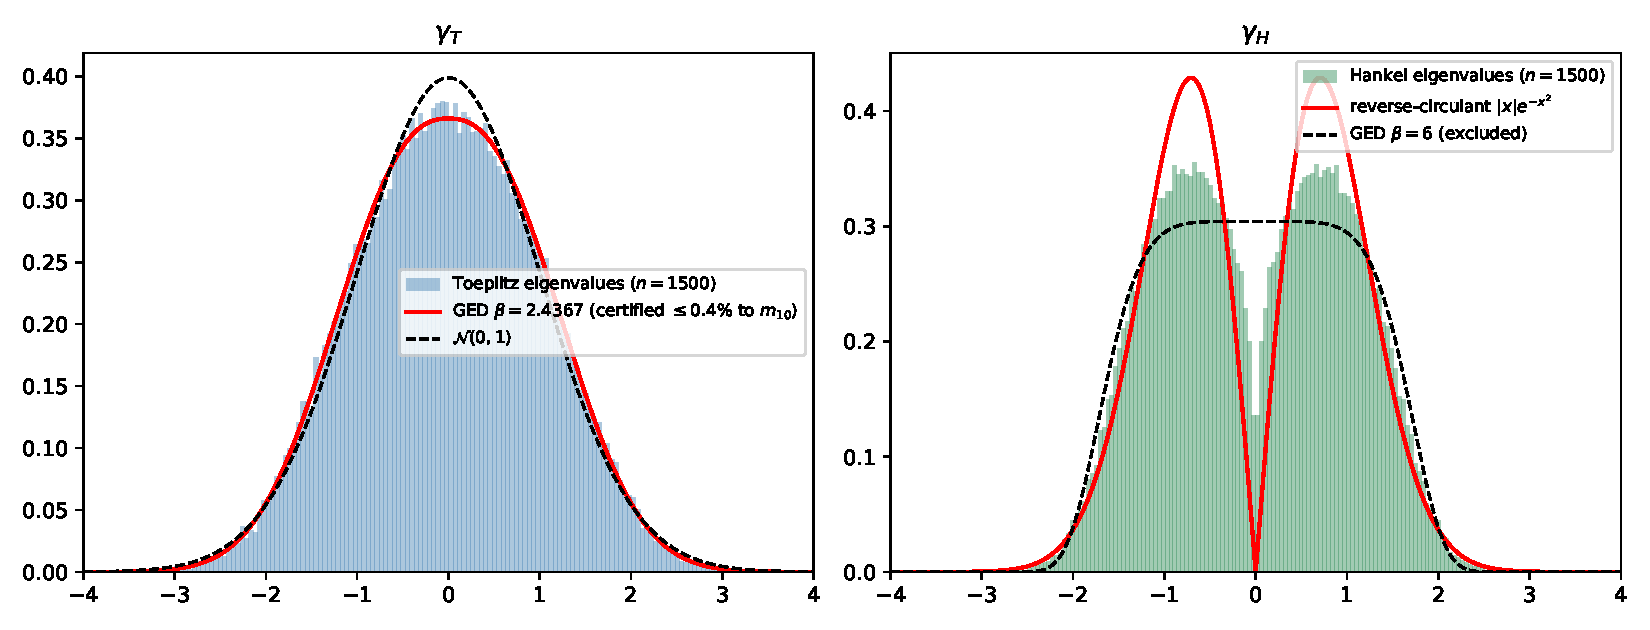
\includegraphics[width=\textwidth]{fig_density}
\caption{Simulated spectral densities ($n=1500$, $60$ repetitions). Left: $\gT$ with
the GED surrogate ($\beta=2.4367$; indistinguishable at this resolution,
provably distinct at order $6$) and the standard Gaussian. Right: $\gH$ (bimodal) with
the reverse-circulant density $|x|e^{-x^2}$ and the excluded GED fit.}
\label{fig:density}
\end{figure}

\section{Reproducibility}\label{sec:repro}
All code (pure Python: \texttt{tk\_core.py}, \texttt{exact\_volume.py},
\texttt{run\_moments.py}, every verification script) and all data (machine-readable
per-orbit exact volumes as JSON) are public at
\begin{center}
\url{https://github.com/yspennstate/toeplitz-hankel-exact-moments}
\end{center}
together with scripts that regenerate every table of this paper from scratch. Every
number in Theorem~\ref{thm:values} is reproducible end-to-end on a laptop; the
values are exact rationals produced by integer-only arithmetic, and the
disputed order ($2k=8$, Toeplitz) is covered by a second, independent exact
implementation (\texttt{brute\_vertices\_check.py}) sharing no code with the first.

\subsection*{Funding}
The research presented in this paper was supported by the European Research Council
(ERC) under the European Union's Horizon 2022 research and innovation programme
(grant agreement No.\ 101041711), by the Simons Foundation, by Heights Labs, by the
Israel Science Foundation (grant number 2258/19) and by the Israel Science Foundation
(ISF Grant 4101/25).

\subsection*{Declaration of generative AI and AI-assisted technologies in the
manuscript preparation process}
During the preparation of this work the author used generative AI tools (large
language model assistants) to assist with drafting, revision and bibliographic
organization. After using these tools, the author reviewed and edited the content as
needed and takes full responsibility for the content of the manuscript.

\subsection*{Declaration of competing interest}
The author declares no competing interests.

\appendix
\section{Complete volume spectra at the highest orders}\label{app:spectra}

\noindent\textbf{Toeplitz, $2k=12$} ($10395$ pairings, $554$ dihedral orbits, $28$
distinct volumes; the $132=\Cat_6$ non-crossing pairings carry volume $1$):
\begin{center}\small
$1\times132$;\ $\tfrac{2}{3}\times495$;\ $\tfrac{1}{2}\times880$;\
$\tfrac{9}{20}\times264$;\ $\tfrac{4}{9}\times66$;\ $\tfrac{2}{5}\times330$;\
$\tfrac{11}{30}\times1452$;\ $\tfrac{61}{180}\times480$;\ $\tfrac{1}{3}\times120$;\
$\tfrac{43}{140}\times4$;\ $\tfrac{383}{1260}\times18$;\ $\tfrac{13}{45}\times840$;\
$\tfrac{2}{7}\times7$;\ $\tfrac{49}{180}\times1800$;\ $\tfrac{19}{70}\times60$;\
$\tfrac{23}{90}\times96$;\ $\tfrac{1}{4}\times396$;\ $\tfrac{313}{1260}\times132$;\
$\tfrac{5}{21}\times102$;\ $\tfrac{71}{315}\times54$;\ $\tfrac{68}{315}\times456$;\
$\tfrac{19}{90}\times234$;\ $\tfrac{22}{105}\times117$;\ $\tfrac{29}{140}\times80$;\
$\tfrac{17}{84}\times82$;\ $\tfrac{509}{2520}\times984$;\
$\tfrac{239}{1260}\times528$;\ $\tfrac{19}{105}\times186$.
\end{center}
Sum: $m_{12}(\gT)=23840/7$.

\medskip
\noindent\textbf{Hankel, $2k=14$} ($5040$ pairings, $260$ orbits, $39$ distinct
volumes; the $429=\Cat_7$ non-crossing pairings carry volume $1$):
\begin{center}\small
$1\times429$;\ $\tfrac{1}{2}\times1001$;\ $\tfrac{11}{30}\times728$;\
$\tfrac{1}{3}\times91$;\ $\tfrac{13}{45}\times455$;\ $\tfrac{49}{180}\times455$;\
$\tfrac{23}{90}\times84$;\ $\tfrac{1}{4}\times190$;\ $\tfrac{5}{21}\times84$;\
$\tfrac{68}{315}\times168$;\ $\tfrac{29}{140}\times28$;\ $\tfrac{17}{84}\times7$;\
$\tfrac{509}{2520}\times504$;\ $\tfrac{239}{1260}\times168$;\
$\tfrac{17}{90}\times14$;\ $\tfrac{59}{315}\times14$;\ $\tfrac{31}{168}\times7$;\
$\tfrac{19}{105}\times84$;\ $\tfrac{5}{28}\times14$;\ $\tfrac{433}{2520}\times7$;\
$\tfrac{1}{6}\times7$;\ $\tfrac{167}{1008}\times14$;\ $\tfrac{59}{360}\times7$;\
$\tfrac{809}{5040}\times7$;\ $\tfrac{1613}{10080}\times28$;\
$\tfrac{1591}{10080}\times56$;\ $\tfrac{197}{1260}\times28$;\
$\tfrac{781}{5040}\times7$;\ $\tfrac{16}{105}\times28$;\
$\tfrac{253}{1680}\times14$;\ $\tfrac{379}{2520}\times42$;\
$\tfrac{1511}{10080}\times42$;\ $\tfrac{367}{2520}\times14$;\
$\tfrac{241}{1680}\times42$;\ $\tfrac{353}{2520}\times56$;\
$\tfrac{349}{2520}\times56$;\ $\tfrac{683}{5040}\times14$;\
$\tfrac{47}{360}\times32$;\ $\tfrac{109}{840}\times14$.
\end{center}
Sum: $m_{14}(\gH)=1331087/720$. Note the leading segments of the two spectra agree
(the shared ``core'' phenomenon of Section~\ref{sec:consequences}).

\medskip
\noindent\textbf{Toeplitz, $2k=14$} ($135135$ pairings, $5283$ dihedral orbits, $70$
distinct volumes; the $429=\Cat_7$ non-crossing pairings carry volume $1$; largest
crossing volume again $\tfrac23\times2002$): the full spectrum is machine-readable in
the repository (\texttt{results/volumes\_T14.json}); its sum is
$m_{14}(\gT)=325719/10$.

\begin{thebibliography}{9}
\bibitem{BDJ} W.~Bryc, A.~Dembo, T.~Jiang,
\emph{Spectral measure of large random Hankel, Markov and Toeplitz matrices},
Ann. Probab. \textbf{34} (2006), 1--38.
\bibitem{HM} C.~Hammond, S.~J.~Miller,
\emph{Distribution of eigenvalues for the ensemble of real symmetric Toeplitz
matrices}, J. Theoret. Probab. \textbf{18} (2005), 537--566.
\bibitem{BoseSen} A.~Bose, A.~Sen,
\emph{Another look at the moment method for large dimensional random matrices},
Electron. J. Probab. \textbf{13} (2008), 588--628.
\bibitem{Maurya} S.~N.~Maurya, \emph{Limiting spectral distribution of Toeplitz and
Hankel matrices with dependent entries}, arXiv:2306.15533.
\bibitem{BoseVish} A.~Bose, P.~Vishwakarma, \emph{Revisiting Toeplitz and Hankel
random matrices via $*$-convergence of circulant-type matrices}, arXiv:2605.16160.
\bibitem{BoseReview} A.~Bose, S.~Chatterjee, S.~Gangopadhyay,
\emph{Limiting spectral distributions of large dimensional random matrices},
J. Indian Statist. Assoc. \textbf{41} (2003), 221--259.
\bibitem{Meckes} M.~Meckes, \emph{On the spectral norm of a random Toeplitz matrix},
Electron. Comm. Probab. \textbf{12} (2007), 315--325.
\bibitem{SV1} A.~Sen, B.~Vir\'ag, \emph{Absolute continuity of the limiting eigenvalue
distribution of the random Toeplitz matrix}, Electron. Comm. Probab. \textbf{16}
(2011), 706--711.
\bibitem{SV2} A.~Sen, B.~Vir\'ag, \emph{The top eigenvalue of the random Toeplitz
matrix and the sine kernel}, Ann. Probab. \textbf{41} (2013), 4050--4079.
\bibitem{ShmaloPR} Y.~Shmalo, \emph{Extreme least singular values of Gaussian row
submatrices and a phase retrieval stability problem}, preprint (2026).
\end{thebibliography}

\end{document}
